\documentclass{../../text-style}

\texttitle{Экосистема open source проектов}

\begin{document}

\maketitle
\thispagestyle{empty}

\section{Введение}

В этой лекции пойдёт речь об инструментах, которые призваны облегчить open source (и не только) разработку --- системы непрерывной интеграции, облачные анализаторы кода, всякие инфраструктурные штуки типа средств планирования и средств общения разработчиков. Все рассматриваемые сегодня инструменты бесплатны для open source и широко используются, поэтому рекомендуются и к использованию в домашках (некоторые даже настоятельно рекомендуются, CI будет обязательна). Обзор, естественно, далеко не полон, таких штук существенно больше, чем будет сегодня рассказано, и даже не факт, что будет рассказано про лучшие --- выбор инструментов, о которых пойдёт речь сегодня, обусловлен прежде всего личным опытом и предпочтениями. Имеет смысл погуглить аналоги и почитать отзывы, потому как этот обзор устарел сразу, как только был написан.

\section{Отступление про сборку из консоли в Windows}

Несколько соображений по поводу сборки из консоли, на случай, если кто-то не умеет. Во-первых, зачем это надо, когда есть привычная IDE, уже должно быть понятно: на CI-системе IDE нет, а если бы была, некому было бы нажимать на кнопки. Ну и вообще, нормальные программисты автоматизируют всё вокруг, а автоматизация --- это прежде всего работа с консольными инструментами. Вот несколько соображений по их поводу.

\begin{itemize}
    \item Консоль под Windows можно запустить, нажав Win-R и набрав cmd в появившемся окне. Либо правым кликом по кнопке <<Пуск>> и там выбрать <<Консоль>>, либо <<PowerShell>>. PowerShell лучше, но немного по-другому работает. Ещё есть Developer Command Prompt --- консоль с настроенными переменными окружения для пользования инструментами Visual Studio из консоли (например, сборки из консоли). Именно её  придётся использовать, если у вас проект не .NET или вообще не установлен .NET SDK. Если .NET SDK есть, то и обычная консоль подойдёт, иначе --- нет.
    \item Основные консольные команды: cd --- переход в указанную папку, dir --- посмотреть содержимое текущей папки, справка по консольным командам: \url{https://ss64.com/nt/syntax.html}.
    \item Есть ещё переменные окружения. Это глобальные переменные, выставляемые для всей операционной системы (либо текущего пользователя) и доступные из скриптов и из программ. Выставляются командой set, например, \mintinline{text}|set x=ololo|, и к ним можно обращаться через \%, например, \mintinline{text}|echo %x%|. Самая интересная переменная окружения, которая всегда установлена --- PATH, это список путей (разделённых точкой с запятой), по которым операционная система ищет исполняемый файл, когда вы набираете команду в консоли. То есть, когда вы пишете dotnet что-то-там, Windows сначала ищет dotnet.exe (или dotnet.bat и ещё несколько других расширений) в текущей папке, если не находит, начинает последовательно перебирать все пути из PATH. Если и там не находит, ругается. Поэтому, если вы хотите, чтобы ваш любимый консольный инструмент (например, python.exe) можно было вызывать, не указывая полный путь до его исполнимого файла, пропишите путь до него в PATH (только аккуратно, не затерев всё остальное). Для редактирования переменных окружения в 10-й Windows есть даже удобный GUI, <<Настройки>> -> <<Системные переменные среды>>.
    \item NuGet Command Line --- утилита для работы с менеджером пакетов NuGet из командной строки, надо ставить отдельно (на CI-серверах обычно предустановлена). NuGet --- это та самая штука, которая подключает и укачивает из интернета при сборке внешние библиотеки, например, библиотеку модульного тестирования. Наличие Nuget Command Line в PATH позволяет делать nuget restore перед сборкой, чтобы избежать ошибок с тем, что библиотеки не найдены.
    \item Небольшая реклама полезных консольных инструментов:
    \begin{itemize}
        \item FAR (\url{https://www.farmanager.com/}) --- File and ARchive manager, незаменимая вещь, хотя выглядит жутковато. Это консоль, но с удобным отображением файлов и папок, возможностью легко и приятно копировать, перемещать, удалять файлы и папки, искать, делать прочие штуки. Имеет встроенный текстовый редактор с синтаксической подсветкой, и главное, командную строку, в которую можно писать консольные команды. Куча полезных хоткеев, запоминание истории команд и истории папок, быстрый переход к папке и т.д. и т.п. В общем, практически must have, и главное, must уметь ей пользоваться.
        \item Chocolatey (\url{https://chocolatey.org/}) --- пакетный менеджер для Windows, наподобие линуксовых apt или brew. Сам качает, устанавливает и поддерживает в актуальном состоянии софт на компе. Ставите Chocolatey, дальше можно писать в консоли что-то в духе choco install git, choco install far, choco install практически что угодно. А поскольку это консольный тул, то его можно вызывать в скриптах, так что можно, например, сделать и выложить на GitHub скрипт, который на голую винду с Chocolatey накатывает весь ваш любимый софт полностью автоматически, и теперь, после того, как вы переустановили Windows, пара команд --- и рабочее окружение настроено и полностью готово к работе. Единственное, что запускать его надо с правами администратора.
    \end{itemize}
\end{itemize}

Главный инструмент работы с C\# в консоли --- это .NET Command-Line Interface (.NET CLI, также известный как просто dotnet). Он умеет фактически всё, что умеет Visual Studio --- создавать проекты, собирать, запускать, добавлять зависимости и т.д. и т.п., при этом ставится вместе с .NET, очень маленький, простой в использовании и бесплатный. Вот основные команды:

\begin{itemize}
    \item dotnet new --- создать новый проект, принимает тип желаемого проекта и может принимать дополнительные параметры, например, <<на каком языке>>. Создаёт проект по шаблону (как VS), то есть по идее сразу работоспособный. Например, dotnet new console создаст вам консольное приложение. Заводите пустую папку, переходите туда вашим любимым консольным тулом, делаете dotnet new --- и оно создаёт проект, называющийся как папка.
    \item dotnet restore --- получить NuGet-пакеты для текущего проекта. Надо запускать каждый раз, когда вы меняли зависимости от сторонних библиотек, получаемых через NuGet.
    \item dotnet build --- собрать проект в текущей папке.
    \item dotnet run --- запустить проект в текущей папке. При необходимости собирает проект. Например, \mintinline{text}{dotnet run -- моиАргументы}. После \mintinline{text}{--} идут аргументы, которые передаются запускаемой программе.
    \item dotnet test --- запустить юнит-тесты для проекта в текущей папке. При необходимости тоже собирает проект.
\end{itemize}

\section{Continuous Integration}

Непрерывная интеграция --- это практика слияния всех изменений по нескольку раз в день, сборки их в известном окружении и запуска юнит-тестов. Стала популярной в начале 2000-х, когда люди заметили, что в современном динамичном мире разделять задачу по разработчикам, ждать несколько месяцев, пока каждый сделает свою часть, а потом пытаться собрать воедино то, что получилось --- плохая идея. Этап интеграции часто становился самым непредсказуемым этапом разработки --- если вам везло, все части просто вставали на свои места и начинали работать вместе, если не везло, половину системы надо было переписывать с нуля. 

Интеграцию проводить тем сложнее, чем дольше времени интегрируемые части разрабатывались независимо. Поэтому самый простой способ сделать интеграцию безболезненной --- минимизировать это время, с месяцев до часов или даже десятков минут. В оригинале непрерывная интеграция была именно методологической штукой, предписывавшей разработчикам двигаться маленькими шажками и вливать всё в мастер (в основную ветку, git тогда ещё не было) каждое сколько-нибудь работающее изменение.

В современном понимании непрерывная интеграция несколько менее радикальна. Она предполагает лишь то, что после каждого коммита изменения должны автоматически проверяться на собирабельность и работоспособность, путём запуска на специально выделенном сервере процесса сборки и юнит-тестов. Зачем --- думаю понятно, во-первых, так можно найти ошибку сразу же, как только она была внесена, во-вторых, сервер непрерывной интеграции становится эталонным окружением, на котором всё точно собирается и работает, и можно посмотреть, как именно. 

Возможна непрерывная интеграция только в том случае, если процесс сборки полностью автоматизирован и воспроизводим. Это не то чтобы проблема, а, скорее, желаемое качество любого нормального проекта. Именно за этим разрабатываются разные консольные инструменты сборки несмотря на то, что IDE сами имеют такую функциональность. Кроме того, всё, что нужно для сборки, должно быть в репозитории. Зато если непрерывную интеграцию удалось наладить, любой новый разработчик, пришедший в проект, может просто получить себе на чистую машину исходники (ну, почти чистую, средства разработки всё-таки надо поставить) и собрать всё одной командой. Это большой шаг вперёд по сравнению с инструкциями по сборке, плясками с бубном и попытками угадать правильные ключи (и правильную версию!) компилятора.

Непрерывная интеграция особенно полезна, если в проекте есть большое количество юнит-тестов, которые можно запустить автоматически. Юнит-тесты обычно запускаются сразу после сборки и если что-то не так, тут же ловят ошибку. Если тестов нет или их мало, проект может собираться, но не работать.

Настраивается непрерывная сборка с помощью механизма <<commit hooks>>, поддерживаемого любой нормальной системой контроля версий. Сервер сборки (а обычно это заранее настроенная виртуалка с установленными компиляторами, системами сборки и клиентом git-а) подписывается на репозиторий, после каждого коммита получает исходники, выполняет сборку, тестирование, сохраняет результаты --- и откатывается до исходного состояния; как правило, просто восстанавливая виртуальную машину из образа или снимка. Это гарантирует, что предыдущие сборки никак не влияют на последующие.

Ещё часто сервер настраивают так, чтобы он извещал всех заинтересованных лиц о статусе сборки --- совершенно точно о проваленных сборках, иногда и об успешных. Делают это все по-разному --- кто-то рассылает письма в рассылки, кто-то постит в Slack/какой-нибудь другой мессенджер, кто-то (все штуки, про которые будет речь далее) выставляет статус коммита на GitHub. Если сборка или юнит-тесты на CI не прошли, принято приостанавливать разработку и чинить то, что сломалось --- пока CI не одобряет последний коммит, новую функциональность не выкладывают. Ситуаций типа <<ну тут есть пара тестов, они и не должны проходить>> также не допускают, иначе можно не заметить серьёзной проблемы.

Раз CI служит истиной в последней инстанции касательно адекватности коммита, то с методологической точки зрения задача не считается выполненной, пока сборка не прошла успешно. Считается невежливым даже уходить домой вечером, если сборка ещё не закончилась --- потому что если она таки не пройдёт, можно прийти с утра и увидеть, что весь офис пытается найти и исправить какой-нибудь дурацкий баг, который вы случайно забыли. А раз так, то билды должны проходить очень быстро --- считается приличным не больше 10 минут, включая запуск юнит-тестов. Для этого используется разделение на компоненты и отдельный билд каждой, параллелизация сборок, а также такая штука, как deployment pipeline.

Основная идея deployment pipeline в том, что раз сборка может быть долгой, можно разбить её на этапы и иметь возможность быстро провести sanity check (и отпустить разработчика домой), а уже потом долго и обстоятельно всё тестировать. Такая сборка настраивается на нескольких машинах, как конвейер --- сначала выполняется собственно сборка, потом запускаются быстрые юнит-тесты, потом собранные бинарники передаются на другую машину, которая запускает долгие тесты (она может это делать, например, раз в сутки, ночью). Если всё хорошо, бинарники передаются на ручное тестирование, а если и там всё хорошо, то на машину, которая зальёт их туда, откуда их получит пользователь. Поэтому и deployment pipeline --- полностью (или почти полностью) автоматизируется весь процесс, от коммита до деплоя у конечного пользователя.

\section{GitHub Actions}

GitHub Actions --- на данный момент практически стандарт де-факто для облачной сборки, поскольку встроена в GitHub и бесплатна для open source-проектов. Облачность хороша тем, что вам не надо искать хост, настраивать виртуалки и всё такое --- всё уже сделано за вас. Чтобы собирать проект и выполнять разные проверки, достаточно просто выложить в репозиторий конфигурацию сборки и включить GitHub Actions в настройках:

\begin{itemize}
    \item В своём репозитории на GitHub идём во вкладку Settings, там Actions, выбираем Allow all actions.
    \item Создаём в корне репозитория папку .github/workflows/.
    \item В нём создаём файл <имя действия>.yml (например, ci.yml).
    \item Описываем процесс сборки согласно \url{https://docs.github.com/en/actions/learn-github-actions/workflow-syntax-for-github-actions}
    \begin{itemize}
        \item Пример и описание линуксовой сборки: \url{https://www.incredibuild.com/blog/using-github-actions-with-your-c-project}
    \end{itemize}
    \item Коммитим-пушим.
    \item Смотрим статус коммита и пуллреквеста.
\end{itemize}

Если всё хорошо, через некоторое время (небольшое, порядка нескольких минут) во вкладке Actions появится статус сборки, например,

\begin{center}
    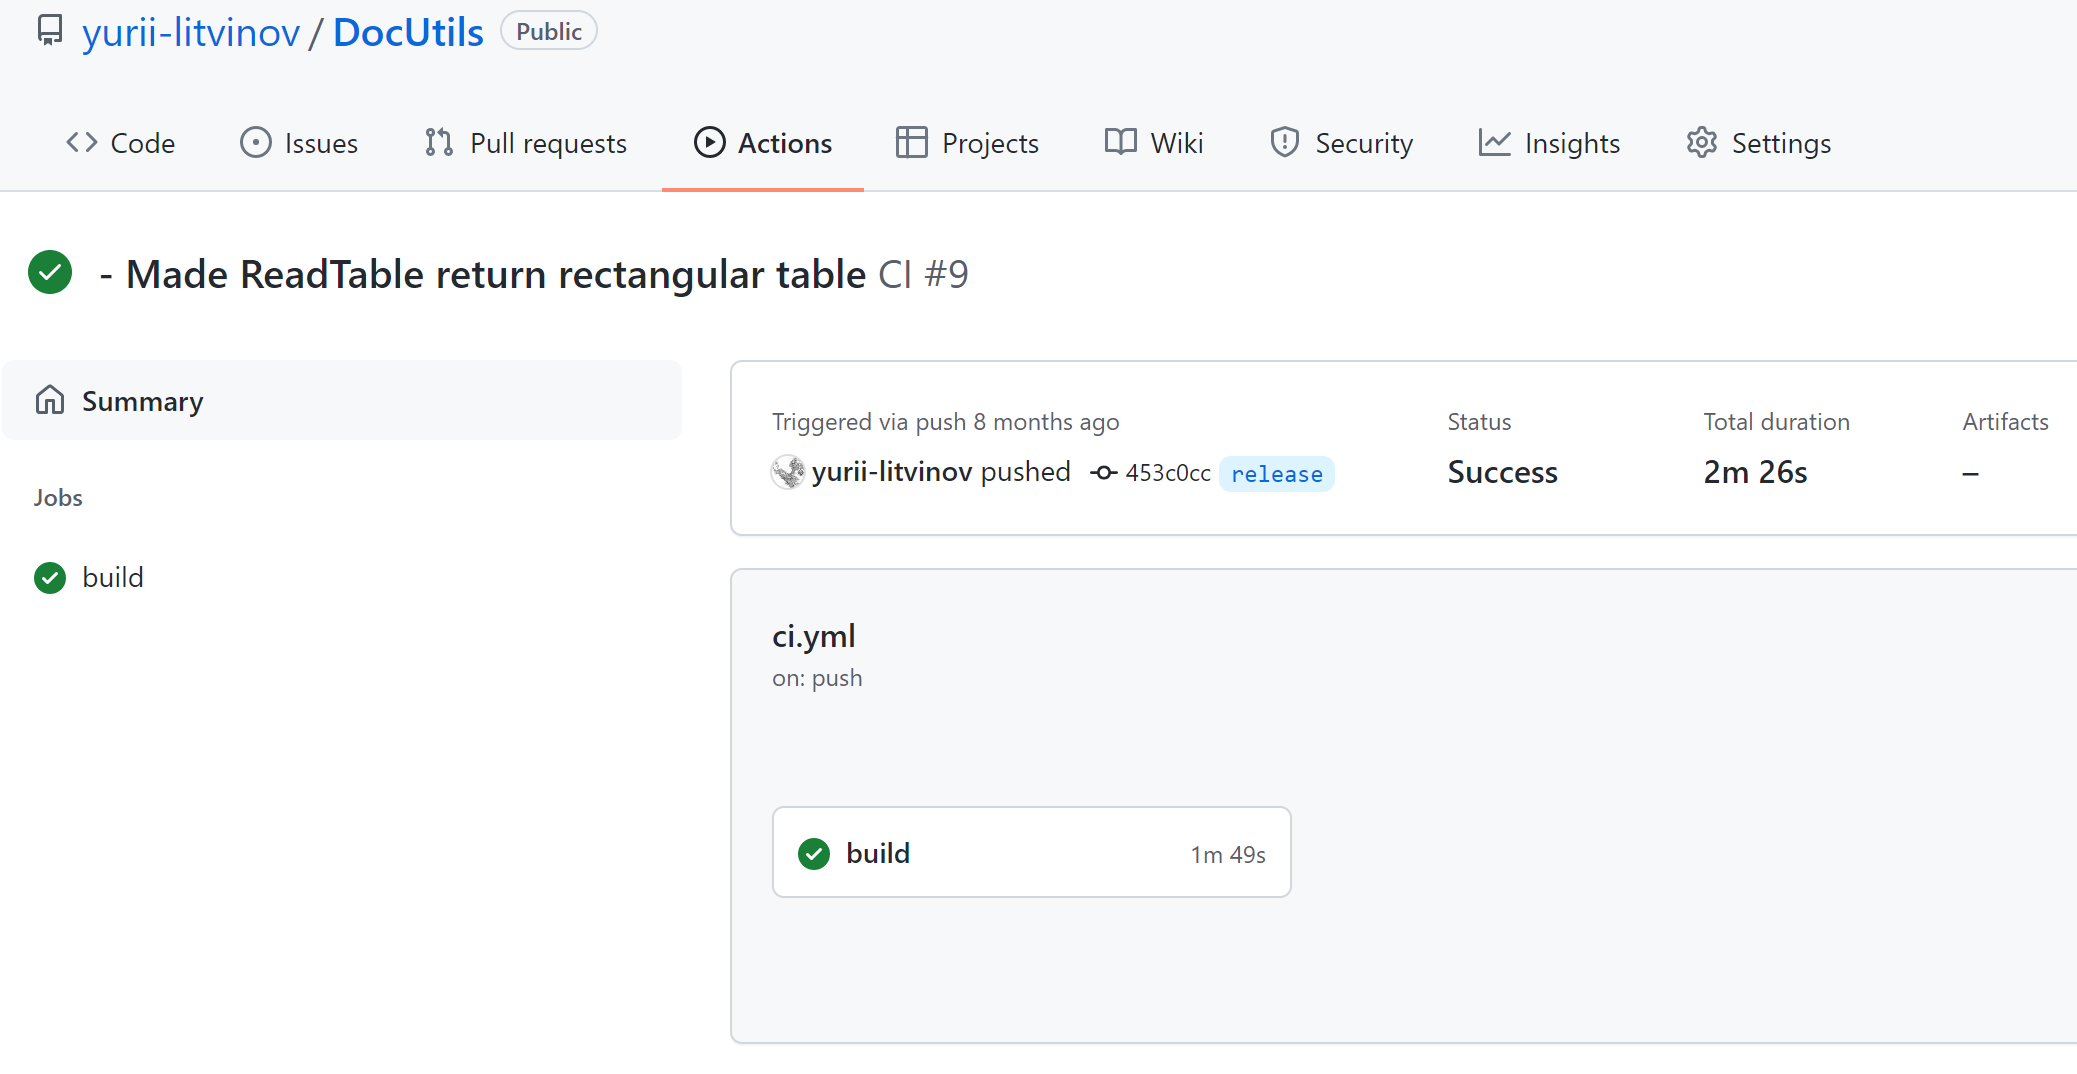
\includegraphics[width=0.9\textwidth]{githubActionsBuildStatus.png}
\end{center}

Также статус сборки будет показываться у каждого коммита в виде зелёной галочки или красного крестика, и у каждого пуллреквеста. Что очень удобно --- если CI не прошёл, сдавать домашку бессмысленно, её точно не зачтут.

\subsection{Примеры конфигурации сборки}

Вот пример конфигурации сборки, обычной для типичного репозитория с домашками (это тот самый ci.yml, упоминавшийся выше, он должен быть в .github/workflows/, при этом папка .github должна быть в корне репозитория, и всё должно называться именно так и лежать именно так, вплоть до написания строчными буквами):

\begin{minted}{yaml}
name: Build
on: [push, pull_request]
jobs:
    build-Ubuntu:
        runs-on: ubuntu-latest
        steps:
            - uses: actions/checkout@v2
            - uses: actions/setup-dotnet@v1
              with:
                  dotnet-version: '6.x'
            - name: Build
              run: For /R %%I in (*.sln) do dotnet build %%I
            - name: Run tests
              run: For /R %%I in (*.sln) do dotnet test %%I
    build-Windows:
        runs-on: windows-latest
        steps:
            - uses: actions/checkout@v2
            - uses: actions/setup-dotnet@v1
              with:
                  dotnet-version: '6.x'
            - name: Build
              run: For /R %%I in (*.sln) do dotnet build %%I
            - name: Run tests
              run: For /R %%I in (*.sln) do dotnet test %%I
\end{minted}

Вот пример более настоящего проекта, когда один проект в репозитории:

\begin{minted}{yaml}
name: CI

on: [push]

jobs:
  build:
    runs-on: windows-latest
    steps:
      - uses: actions/checkout@v2
      - uses: actions/setup-dotnet@v1
        with:
          dotnet-version: '6.x' 
      - run: dotnet build 
      - run: dotnet test
\end{minted}

И пример репозитория, откуда он был взят: \url{https://github.com/yurii-litvinov/DocUtils}.

Тут name: CI --- это имя Workflow-а (вместо CI может быть что угодно, это потом будет отображаться во вкладке Actions c результатами сборки). on --- это событие, запускающее процесс, в данном случае по любому push-у в репозиторий. jobs --- это список работ, каждый job работает на своей виртуальной машине. build --- это имя работы, может быть произвольным. runs-on --- это образ виртуалки (на самом деле, Docker-контейнера вроде), на котором запускать работу. steps --- это шаги сборки. uses --- это Action-ы, из которых состоит сборка, with --- их параметры. run --- это скрипты, то есть обычные консольные команды, которые последовательно исполняются в процессе сборки.

\subsection{Основные концепции}

Расскажем, что происходит в конфигурации сборки. GitHub Actions --- это на самом деле механизм, который позволяет реагировать на некое \emph{событие} (Event), запуская некие \emph{работы} (Jobs). Работы состоят из \emph{шагов} (Step), которые могут быть либо скрипт, либо Action:

\begin{center}
    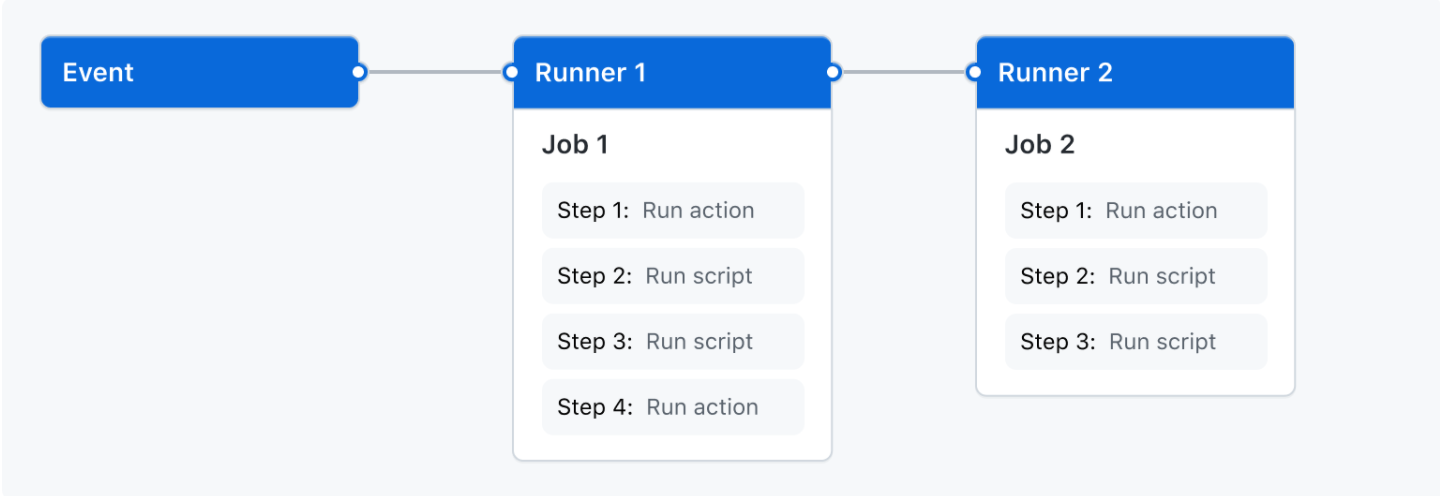
\includegraphics[width=0.7\textwidth]{githubActionsWorkflow.png}
\end{center}

Скрипт --- это обычная консольная команда, синтаксис которой зависит от выбранного образа (того, что написано в runs-on). Action --- это произвольный код (по сути, отдельное приложение), который можно подключить к Workflow, чтобы он делал какую-то потенциально сложную работу. Есть куча готовых Action-ов, как от самого GitHub, так и сторонних. Action, по сути, строительный блок, из них можно собирать сложные сценарии сборки. Также можно переиспользовать и сами Workflow-ы, но это имеет довольно ограничений, чтобы предотвратить возможность выполнения вредоносного кода и кражу данных.

\subsection{Тонкости конфигурации}

Для всех CI-систем, GitHub Actions в том числе, важна возможность выставлять переменные окружения, поскольку через них выполняется конфигурирование довольно многих программ (например, в следжующем семестре, надеюсь, будет про веб-приложения и сервер Kestrel, который управляется в том числе переменными окружения). В GitHub Actions это делается через команду env:

\begin{minted}{yaml}
env:
    DAY_OF_WEEK: Monday

jobs:
    greeting_job:
    runs-on: ubuntu-latest
    env:
        Greeting: Hello
    steps:
        - name: "Say Hello Mona it's Monday"
        if: ${{ env.DAY_OF_WEEK == 'Monday' }}
        run: echo "$Greeting $First_Name. Today is $DAY_OF_WEEK!"
        env:
            First_Name: Mona
\end{minted}

env выставляет переменные окружения для контекста, в котором они объявлены, например, DAY\_OF\_WEEK выставляется для всего Workflow, Greeting --- только для greeting\_job, First\_Name только для Step-а. Используются переменные окружения как обычные переменные окружения в шелле. В примере выше речь про Ubuntu и шелл Bash, там переменная окружения подставляется через <<\$>>. В Windows используется PowerShell, nам подстановка выполняется как \mintinline{text}.

Переменные окружения можно использовать для конфигурации сборки довольно топорным способом --- например, записывая туда проекты, которые надо собрать. А чтобы иметь возможность перебирать несколько разных значений переменных, есть понятие <<матрица сборки>>:

\begin{minted}{yaml}
runs-on: ${{ matrix.os }}
strategy:
  matrix:
    os: [ubuntu-18.04, ubuntu-20.04]
    node: [10, 12, 14]
steps:
  - uses: actions/setup-node@v2
    with:
      node-version: ${{ matrix.node }}
\end{minted}

Тут определяются <<переменные окружения>>\footnote{Раскрытие этих переменных выполняется не шеллом, а самой системой сборки, поэтому и синтаксис оператора подстановки такой необычный --- \mintinline{text}|${{ matrix.os }}|.} matrix.os и matrix.node, и система сборки последовательно перебирает все их значения, указанные в матрице, запуская отдельные job-ы для каждой пары значений (почему и матрица --- суммарное количество сборок определяется декартовым произведением всех возможных значений, то есть тут будет сборка под две разные версии Ubuntu каждой из трёх версий Node.js). 

Зачем это может быть полезно? Вспомните первый пример конфигурации сборки, где два абсолютно одинаковых скрипта собирали систему под Windows и под Linux. С помощью матрицы сборки из одной переменной os с двумя значениями скрипт можно сделать вдвое короче. А потом ещё и можно будет легко добавить сборку под macOS. Вообще, собирать и тестировать под разными операционными системами --- очень хорошая практика, поскольку кроссплатформенность таит в себе немало сюрпризов, но вместе с тем в большинстве случаев очень желательна.

\subsection{Дополнительные возможности}

Ещё GitHub Actions умеет делать следующие штуки (мы тут их просто перечислим, подробности --- в документации, непосредственно в домашке они не пригодятся).

\begin{itemize}
    \item Секреты --- возможность использовать внутри Workflow конфигурационные параметры, которые нельзя выкладывать в общий доступ. Например, ваш пароль от вконтакта, куда Workflow будет постить об успешной сборке, или, более реалистично, пароль от сервера, на который надо выполнить развёртывание после сборки. Секреты задаются через пользовательский интерфейс GitHub в настройках репозитория, и в самом репозитории не хранятся (то есть не имея доступа к вашему аккаунту враги его не украдут). Использовать секреты можно как обычные <<переменные>> из матрицы сборки: \mintinline{yaml}|super_secret: ${{ secrets.SUPERSECRET }}|
    \item Кеширование промежуточных результатов --- сборку можно разбить на фазы и сказать GitHub Actions не удалять результаты предыдущей фазы, чтобы, например, в процессе сборки не выкачивать ещё раз четырёхгиговый образ чего-нибудь. Кешировать собираемые бинарники обычно плохая идея, потому что может показаться, что всё ок, только потому, что в прошлый раз собралось, а сейчас старое не удалилось. 
    \item Автоматическое развёртывание --- результаты успешной сборки могут заливаться куда-то типа продакшн-сервера. В частности, можно собирать документацию к коду и автоматически загружать её на github-pages.
    \item Проверка стиля кодирования, статический анализ кода и т.п., что полезно как само по себе, так и делает осмысленной сборку даже того, что и собирать, в общем-то, не надо --- код на Python, например. Только обратите внимание, что если собственно сборку стоит проводить под разными операционными системами, то проверять стайлгайд надо только под одной. Так что такие вещи обычно делаются отдельным Workflow-ом.
    \item Можно иметь несколько Workflow-ов в одном репозитории. Просто кладёте несколько .yml-файлов с разными названиями в папку workflows, и всё.
\end{itemize}

\section{AppVeyor}

Ещё один пример облачной CI-системы --- это AppVeyor (\url{https://www.appveyor.com}). Довольно удобный веб-интерфейс для конфигурирования, куча документации, но, естественно, несколько ограниченные возможности по сравнению с тем, что можно сделать руками (например, ограничение времени билда в что-то около часа). AppVeyor бесплатен для open source проектов и при этом довольно прилично работает, поэтому очень популярен в мире разработки для Windows.

AppVeyor собирает проект на чистой виртуальной машине под Windows Server 2019, есть поддержка и сборки под Linux. Предустановлены инструменты сборки --- Visual Studio 2019, .NET Core, nuget, консольные инструменты для сборки, компиляторы и интерпретаторы других языков (Python, Java и т.д.) конечно, есть git. Интегрируется с GitHub (как в плане настройки сборки в пару кликов из AppVeyor, так и в плане показа статуса сборки у каждого коммита и пуллреквеста), умеет постить результаты в Slack. В качестве системы сборки по умолчанию используется MSBuild --- консольный инструмент сборки от Microsoft. Но можно сконфигурировать сборку самостоятельно, указав хоть MinGW для сборки исходников на C++.

Окружение сборки (зависимости, переменные окружения и т.д.) можно настроить из конфигурационного файла, который выкладывается в репозиторий с исходниками, либо настройками самого AppVeyor-а, либо вручную из скрипта сборки. Скрипт может писаться как прямо в конфигурационном файле, так и отдельно, и тогда из конфигурационного файла он просто запускается. На самом деле, в самых простых случаях (если в репозитории одно решение, лежащее прямо в корне и не требующее ничего, кроме собственно сборки), скрипт можно вообще не писать, настройки по умолчанию всё сделают сами.

\subsection{Настройка сборки}

Для того, чтобы всем этим пользоваться, сначала нужно установить commit hook на GitHub. Это проще всего попросить сделать сам AppVeyor --- идём на \url{https://www.appveyor.com}, логинимся под своим GitHub-овским аккаунтом, жмём <<добавить репозиторий>>, выбираем нужный репозиторий, жмём кнопку <<включить>> и, собственно, всё. При логине GitHub может попросить для AppVeyor права на просмотр списка репозиториев, при подключении репозитория --- права на установку commit hook-а, надо согласиться.

Дальше надо добавить файл appveyor.yml в корень репозитория. Это тот самый конфигурационный файл, о котором упоминалось выше. Можно пустой, если значения по умолчанию вас устраивают. По умолчанию AppVeyor будет собирать Visual Studio 2019, при этом он попытается найти файл .sln в корне репозитория и запустить на него MSBuild.

Коммитим это всё и пушим --- это инициирует процесс сборки. Теперь любой коммит и пуш заставят AppVeyor снова собирать всё с нуля. Это не очень правильно, если вы коммитите только изменения в документации или подредактированные картинки, поэтому AppVeyor (и другие CI-системы) умеет игнорировать коммиты, в комментарии к которым встречается строка <<[ci skip]>>. Вообще, то, что AppVeyor бесплатный --- не повод его безжалостно эксплуатировать, так что использовать <<[ci skip]>> рекомендуется, но использовать его для коммитов, которые таки могут сломать сборку --- не следует.

По окончании сборки AppVeyor сообщит о статусе на GitHub, результаты будут видны у каждого коммита и в пуллреквесте (в пуллреквесте аж два --- сборка ветки, из которой делался пуллреквест, и сборка мерджа из пуллреквеста в мастер, если там нету конфликтов). Выглядит это примерно так:

\begin{center}
    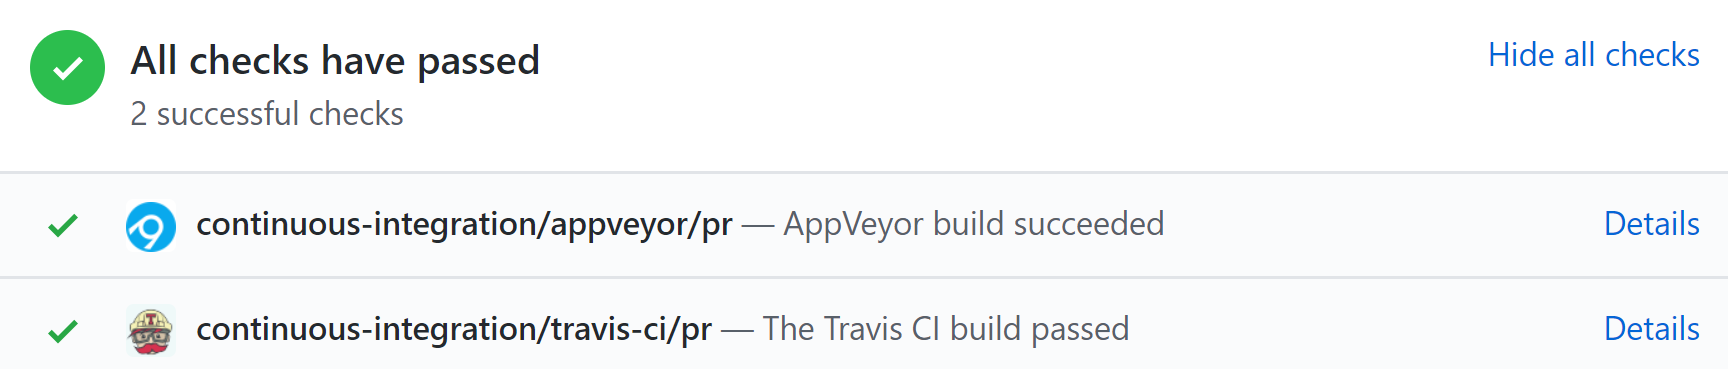
\includegraphics[width=0.7\textwidth]{appVeyorSuccess.png}
\end{center}

Пример конфигурационного файла:

\begin{minted}{yaml}
image: Visual Studio 2022

before_build: 
    - nuget restore myCoolHomework/Homework.sln

build: 
    project: myCoolHomework/Homework.sln

test_script: 
    - dotnet test myCoolHomework/Homework.sln
\end{minted}

Перед началом сборки мы получаем все nuget-пакеты, от которых зависит наше решение, затем запускается собственно сборка, затем, в случае успешной компиляции, запускаются юнит-тесты командой dotnet test.

\section{CodeCov}

Помимо CI, при разработке используется ещё куча облачных инструментов. Следующая штука, которую хочется показать --- это средство для анализа тестового покрытия CodeCov (\url{https://codecov.io/}). На самом деле, эта штука сама тестовое покрытие считать не умеет, и даже тесты не исполняет, она просто использует функциональность, которая и так есть в компиляторах или библиотеках по подсчёту строк кода, исполнявшихся во время тестового прогона. CodeCov просто красиво её визуализирует и показывает прямо на GitHub (комментирует пуллреквест информацией о том, как изменилось бы тестовое покрытие, если бы пуллреквест был принят). Например, для C\# используется OpenCover, для Java (Kotlin, Scala) используется библиотека JaCoCo, для C++/gcc --- ключ <<-coverage>>, встроенный в компилятор.

Как подключить CodeCov к сборке, написано хорошо и подробно в документации, но вот пример того, как это делается из AppVeyor:

\begin{minted}{yaml}
image: Visual Studio 2015

before_build:
- nuget restore
- choco install opencover.portable
- choco install codecov

build:
  project: CodecovProject.sln
  verbosity: minimal

test_script:
- OpenCover.Console.exe -register:user -target:"%xunit20%\xunit.console.x86.exe" -targetargs:".\MyUnitTests\bin\Debug\MyUnitTests.dll -noshadow" -filter:"+[UnitTestTargetProject*]* -[MyUnitTests*]*" -output:".\MyProject_coverage.xml"
- codecov -f "MyProject_coverage.xml
\end{minted}

Правда, тут с XUnit, но несложно переделать на вашу любимую библиотеку юнит-тестирования.

Вообще, CodeCov хорош для того, чтобы понимать, на что именно надо писать тесты и следить, чтобы тестовое покрытие не ухудшалось. Однако надо помнить, что даже 100\% тестовое покрытие не говорит, что в вашем коде нет ошибок. Зато практика показывает, что если метод не покрыт тестами, он, скорее всего, не работает.

\section{Codacy}

Ещё одна полезная штука --- полноценный облачный статический анализатор кода Codacy (\url{https://www.codacy.com/}). На самом деле, это один из многих подобного рода инструментов, но конкретно он один из самых старых и развитых. Codacy умеет искать сразу много типичных ошибок в коде: потенциальные баги, стайлгайд, мёртвый код, проблемы с производительностью и т.д. При этом поддерживается много языков, в том числе C\#, C++, Java, Kotlin, Python, Scala. Codacy очень настраиваема, ей можно сказать, на что ругаться, на что нет, включив/выключив более сотни разных проверок. Может быть очень полезной штукой, но требует некоторых усилий по автоматизации, поэтому не так популярна, как более простые штуки типа BetterCodeHub, которые ничего толком не умеют, но легко интегрируются.

\section{Инструменты планирования}

Теперь немного про инструменты, которые сами с кодом ничего не делают, а помогают с сопутствующими задачами --- управлением проектом и коммуникациями. Первый инструмент, о котором вы, наверное, и сами слышали --- это Trello (\url{https://trello.com/}). Это легковесный инструмент планирования, реализованный как веб-приложение, бесплатный в базовом варианте и используемый не только в IT-сфере, но и везде, где надо что-то организовать, спланировать и упорядочить (вплоть до списка покупок в магазине).

Концептуально Trello представляет собой набор \textit{досок}, каждая доска состоит из \textit{списков}, каждый список состоит из \textit{карточек}. Карточки можно перетаскивать из списка в список, комментировать, снабжать тэгами, делать там списки (в том числе, TODO-списки, откуда можно вычёркивать сделанное), назначать им ответственных, дедлайны, прикладывать картинки и т.д. Типичная организация списков для IT-проектов --- это классические TODO, Doing, Done плюс возможные варианты типа Testing, Designing и т.д. Карточка соответствует одной короткой задаче и перетаскивается между списками. Например, член команды хочет взять себе задачу --- он записывает себя в карточку ответственным и перетаскивает её в Doing, остальные члены команды видят, что задача взята.

Trello не стоит использовать для стратегического планирования, потому что если карточек пара десятков, то ещё ладно, а если у вас взрослый проект с более чем сотней запросов от пользователей, багов и фич, которые надо сделать, то Trello использовать тяжеловато, потому как в карточках будет сложно ориентироваться. Тем не менее, Trello хорош для тактического планирования и отслеживания задач --- например, задач одной итерации большого проекта. Если проект маленький, то Trello идеален.

Более тяжеловесный инструмент планирования --- Pivotal Tracker (\url{https://www.pivotaltracker.com}). Он создавался уже конкретно для разработки ПО, даже более специфично --- для разработки ПО по методологии Scrum. Вообще, Scrum --- это самая популярная нынче из Agile-методологий, по которой разрабатываются практически все проекты сейчас (точнее, как правило, говорят, что разрабатываются, но на самом деле часто от методологи отступают). Методологические подробности будут в курсе <<Разработка ПО>>, а нам сейчас важно, что проект разрабатывается короткими (от недели до месяца) итерациями, команда поддерживает список задач --- так называемый \textit{бэклог}, специально выделенный человек в команде приоритизирует задачи, двигая их вверх-вниз по бэклогу, вся команда оценивает задачи в условных единицах. Есть понятие <<скорость команды>> --- сколько условных единиц команда успевает сделать за одну итерацию. На текущую итерацию отбираются задачи из самого верха бэклога так, чтобы их суммарная оценка соответствовала скорости команды, они фиксируются на итерацию и команда начинает их делать. В Scrum нет тимлида, каждый член команды может сам взять себе задачу и начать её делать. В конце итерации проводится \textit{демо} с презентацией текущих результатов заказчику, либо очередной релиз.

Pivotal Tracker всё это поддерживает. Внешне всё выглядит как в Trello --- есть проект, в нём списки с задачами. Но списка всего три --- Icebox (что было бы неплохо сделать вообще, рано или поздно), Backlog (это уже оцененные и запланированные задачи) и Current (это задачи на текущую итерацию). Задачи можно оценивать в условных единицах, по шкале либо от 0 до 3, либо по фибоначчиевой шкале (0, 1, 2, 3, 5, 8), выбирается в настройках проекта. Задачи имеют тип --- feature, bug, chore (это разные рефакторинги и прочая деятельность по поддержанию кода, которая непосредственной пользы заказчику не приносит), и статус --- Unstarted, Started, Finished, Delivered, Accepted/Rejected, задачи двигаются по фиксированному жизненному циклу от Unstarted к Accepted. При этом автоматически считается скорость команды --- Pivotal Tracker ведёт статистику, сколько условных единиц функциональности было закрыто за итерацию, так что за несколько итераций получается довольно точная оценка реальной скорости команды. При этом на скорость влияют только задачи типа feature --- что реально полезного для заказчика команда успевает сделать за итерацию. Так что если команда целыми днями рефакторит код, чтобы довести его до совершенства, или исправляет свои баги, то скорость её будет низка и планировать много фич на итерацию Pivotal Tracker не позволит (конечно, его можно переубедить, скорость можно прописать вручную, да и задачи назначить на итерацию вручную, но он по крайней мере покажет, что вас может ждать провал). По моему личному опыту, через полгода аккуратного пользования Pivotal Tracker-ом он может предсказывать сроки выполнения этапов проекта с чудовищной точностью --- до плюс-минус пары дней при планировании на полгода. Разные отпуска/болезни/праздники, неточности оценок задач и разные тормозящие факторы усредняются (довольно быстро, на самом деле), и если в команде не происходит больших перемен, даже грубые оценки в среднем дают очень точный результат.

Есть поддержка релизов --- задачу можно пометить как релиз и назначить ему дедлайн, тогда Pivotal Tracker будет предупреждать, если считает, что с существующими запланированными до него задачами релиз не уложится к дедлайну. Есть тэги, по которым можно группировать и искать задачи. Есть epic-и --- это большие задачи, разделяемые на несколько подзадач, и прогресс по epic-у отслеживается по прогрессу по задачам, которые в него входят.

Pivotal Tracker ещё умеет некоторую аналитику --- например, рисовать \textit{burndown chart}-ы. Это график того, как закрываются задачи во время итерации --- по горизонтальной шкале откладывается время, по вертикальной --- количество условных единиц, которые ещё осталось сделать. Можно следить за поведением кривой <<сжигаемых>> в ходе разработки условных единиц, в начале итерации она должна быть где-то высоко, но в конце достичь нуля. Если кривая выше, чем надо, можно бить тревогу.

\section{Средства коммуникации}

Средства коммуникации проектной команды тоже на удивление важны в процессе разработки. Тут на самом деле обычно используется что угодно --- чаще всего почта, Skype, разные корпоративные мессенджеры (Microsoft Lync, который уже помер, Mattermost, который вполне жив). Некоторые пользуются и мессенджерами общего назначения, мы в былые времена пользовались Jabber-ом, затем перешли на Telegram. Такие мессенджеры не очень удобны в том плане, что лучше не смешивать деловое и личное общение, к тому же специализированные штуки имеют полезную функциональность типа возможности расшарить рабочий стол (хотя тут TeamViewer доминирует), подсветки кода, интеграции с багтрекером и системой контроля версий --- всё это обычные бытовые мессенджеры, как правило, не умеют.

Тут хотелось бы упомянуть средства, популярные в open source-мире --- Slack и Gitter. Они довольно легко интегрируются с CI и системами контроля версий, умеют синтаксическую подсветку кода, вложения, отображение картинок и т.д. Gitter в каком-то смысле более открыт --- по умолчанию не требует авторизации, чтобы читать сообщения, поэтому его часто используют для общения с сообществом, когда заинтересованных людей может быть много. Slack имеет понятие <<команда>> и по умолчанию никого извне не пускает, поэтому он популярен для более закрытых проектов, тем не менее, в open source его тоже используют. У Slack несколько получше с интеграцией с разными инструментами, но несколько похуже со скоростью работы (особенно десктопного клиента).

\section{Встроенные средства GitHub}

На самом деле, GitHub, которым вы и так пользуетесь, сам умеет очень многое. Во-первых, GitHub Issues --- встроенный багтрекер, можно включить в настройках для любого репозитория. По сравнению с более взрослыми багтрекерами его возможности довольно ограничены (нет жизненного цикла бага, кучи полей, которыми обычно пользуются, вложенных задач и т.д.), но много чего он всё-таки умеет: майлстоуны с возможностью привязывать к ним задачи и определять дедлайны, метки на багах (с помощью которых на самом деле симулируются и жизненный цикл бага, и всякие пол типа priority, которые багтрекерами обычно поддерживаются <<из коробки>>),  возможность закрывать баги автоматически (если в сообщении коммита есть <<close>> или <<fix>> и \#<номер бага>). Для типичного open source-проекта багтрекер GitHub-а вполне ок, а то, что его не надо настраивать и он достаточно прост, чтобы люди со стороны могли писать вам баги --- дополнительные очки в его пользу (кстати, для обеспечения последнего можно определить шаблоны багов в markdown, тогда при создании нового бага будет сразу создаваться баг по шаблону). Обращаю внимание, что пуллреквест тоже считается Issue, попадает в GitHub Issues и ведёт себя как обычный баг --- его можно открывать/закрывать, назначать ответственного, ставить тэги и т.д., и даже ссылаться в коммитах и других issue через символ \#.

GitHub Projects --- инструмент планирования, в плане функциональности нечто среднее между Trello и Pivotal Tracker. Там тоже есть списки и карточки, которые можно перекладывать между списками, но при этом карточки могут быть привязаны к багам из GitHub Issues. На один репозиторий может быть несколько проектов на GitHub Projects.

GitHub Wiki --- викистраницы, куда можно выкладывать полезную информацию о проекте. Включаются в настройках репозитория, редактируются с использованием Markdown (GitHub flavored, так что там тоже можно ссылаться на баги через решётку, делать красивую синтаксическую подсветку для разных языков и т.д.). Ещё, кстати, GitHub Wiki --- это тоже гитовый репозиторий, так что, во-первых, он ведёт историю ваших изменений, во-вторых, его можно склонит и редактировать локально.

GitHub Pages --- хостинг для статических сайтов. Хостит HTML с JavaScript, которы берёт либо из ветки gh-pages проекта, либо из отдельного репозитория, смотря как настроите. Сайту выделяется доменное имя <<<имя проекта>.github.io>> (бесплатно). Многие проекты таким образом хостят свою документацию, как пользовательскую, так и техническую. 

\section{Авторское право}

Последний, но немаловажный аспект, касающийся open source --- это авторское право. На самом деле это вообще часто забываемый, но весьма важный при разработке ПО вопрос. Дело в том, что даже если код лежит на GitHub и типа в свободном доступе, его далеко не всегда можно переиспользовать в своих проектах. Вообще, международное (и, соответственно, российское) законодательство устроено так, что плодами интеллектуальной деятельности легально можно пользоваться только в том случае, если автор это явно разрешил. Поэтому если вы скопипастили кусок кода с чьего-то репозитория без лицензии в свой проект, актор может вас засудить за кражу интеллектуальной собственности. Так что просто код на GitHub --- это не совсем open source.

Немного подробнее про результаты интеллектуальной деятельности и авторское право. Бывают исключительные и личные неимущественные права. Личные неимущественные права --- это право называться автором произведения, право заявлять, что вы автор и т.д., личные неимущественные права неотчуждаемы --- то есть их нельзя передать и нельзя забрать. Если ваш работодатель пишет в трудовом договоре, что вы не имеете права говорить, что вы писали этот код, этот пункт трудового договора может быть признан недействительным, поскольку противоречит законодательству. Личные неимущественные права называются неимущественными, поскольку всё равно никакого дохода автору не приносят.

Исключительные права можно передать. Исключительные права --- например, право пользоваться произведением, право воспроизводить, модифицировать, продавать и т.д. и т.п. Мало кто знает, что и личные неимущественные права, и исключительные права начинают действовать в момент создания произведения, и принадлежат автору произведения, никакой регистрации или юридического оформления прав не требуется. Единственное, но очень важное исключение --- если произведение создано по служебному заданию, исключительные права на него принадлежат работодателю, так что написать плагин для IDEA в JetBrains и отсудить у JetBrains пару миллионов за то, что они им пользуются, не получится. Обычно это явно прописано в трудовом договоре, но даже если нет, то это всё равно есть в законе об авторском праве. Знаменитый знак копирайта \textcopyright служит только для информирования о правах и не требуется для их существования (то есть если у вас нигде не написано \textcopyright, это никак не влияет на ваши права на произведение). Да, просто кусок кода --- это тоже произведение и тоже охраняется законом об авторском праве.

Некоторая тонкость в том, что соавторы владеют произведением в равной степени, если произведение невозможно явно разделить между ними. Так что если кто-то закоммитит в ваш проект пару строк кода, он становится таким же автором, как и вы, со всеми вытекающими последствиями --- вам надо будет спрашивать согласие соавтора на передачу исключительных прав (в том числе, продажу или смену лицензии).

И ещё одна тонкость --- идея не охраняется, охраняется её физическое выражение. Люди, бегающие и кричащие, что у них есть замечательная идея для стартапа, с точки зрения законодательства на самом деле не имеют ничего. И неспроста --- от идеи до реализации большой путь, и если у вас только идея, то это ещё ничего не значит. Зато если вашу замечательную идею украдут и сделают стартап раньше вас, то законы вас не защитят.

Лицензия --- это на самом деле юридически правильный способ передать часть прав на произведение. Если вы хотите, чтобы вашим кодом всё-таки пользовались, лицензия вам необходима, благо GitHub предлагает выложить лицензию из набора популярных при создании репозитория, да ещё и объясняет, какая вам больше подойдёт. Пример лицензии ---<<Do what the **** you want to public license>> (WT*PL\footnote{https://en.wikipedia.org/wiki/WTFPL}), которая звучит примерно так:
\begin{minted}{text}
DO WHAT THE **** YOU WANT TO PUBLIC LICENSE
                   Version 2, December 2004
 
Copyright (C) 2004 Sam Hocevar <sam@hocevar.net>

Everyone is permitted to copy and distribute verbatim or modified
copies of this license document, and changing it is allowed as long
as the name is changed.
 
           DO WHAT THE **** YOU WANT TO PUBLIC LICENSE
  TERMS AND CONDITIONS FOR COPYING, DISTRIBUTION AND MODIFICATION

 0. You just DO WHAT THE **** YOU WANT TO.
 \end{minted}

К несчастью, <<Want to>> может включать в себя патентование произведения и подачу в суд на автора за нарушение патента (и такие дела реально практикуются патентными троллями), поэтому обычно лицензии более длинны и унылы, даже если хотя сказать примерно то же самое. Кстати,в России и Европе программы не патентуют, в США --- да. В России зато можно получить свидетельство о регистрации программы для ЭВМ, это не очень сложная бюрократическая процедура, которая ничего не даёт, кроме плюс пары баллов при поступлении в магистратуру СПбГУ и возможности формально доказать своё авторство, если вы стали жертвой тролля, пытающегося похитить вашу интеллектуальную собственность.

Общее правило таково, что каждый нормальный open source-проект должен иметь лицензию. Так что начиная с сегодняшнего дня в домашке лицензия обязательна.

Часто используемые open source-лицензии:

\begin{itemize}
    \item GPL, LGPL. GPL вирусная, поэтому использовать её, внезапно, плохая практика. Она создавалась, чтобы подбодрить развитие свободного ПО, поэтому содержит фразу, что ПО, использующее ПО под GPL, само должно быть лицензировано под GPL. В светлом мире GPL-апологетов в конечном итоге всё будет лицензировано под GPL, так что эта фраза не будет иметь значение. В суровой реальности же это очень мешает, потому что серьёзные компании не используют GPL как лицензию, следовательно, весь код, лицензированный под GPL, для них просто не существует. Есть LGPL (Library- или Light-), разрешающая линковаться к GPL-коду, не <<заражаясь>> GPL-лицензией, но включать GPL- код как код всё так же не позволяющая (беда C++никам с их заголовочными файлами). Кстати, есть распространённое заблуждение, что код под GPL должен распространяться бесплатно --- это неправда, лицензия требует лишь, чтобы тот, кому вы продали бинарные файлы, мог получить и код, и имел бы право его модифицировать (при условии, что модификации тоже будут под GPL). Есть ещё Affero GPL, которая касается веб-приложений и требует, чтобы если приложением можно пользоваться по сети, должно быть можно получить его код (GPL такого требовать не могла, потому что у веб-приложений формально бинарники никому не передаются).
    \item MIT License --- разрешающая лицензия, не обладает вирусностью GPL, разрешает пользоваться кодом в том числе и в проектах с другими лицензиями (вклчая коммерческие). Запрещает лишь <<воровать>> интеллектуальную собственность, например, объявив себя единственным обладателем прав на продажу проекта.
    \item Apache License 2.0 устроена примерно как MIT License, но может применяться пофайлово, а не ко всему проекту целиком, и имеет ряд тонкостей, касающихся патентов. Apache License считается более длинной и тяжёлой в применении (она обычно подразумевает наличие шапки с краткой формой лицензии в каждом файле), но более юридически аккуратной, поэтому всенародно любима.
    \item BSD License (в разных вариантах) --- тоже разрешающая лицензия, короткая и по делу.
    \item The Unlicense --- явная передача произведения в Public Domain. Public Domain (или общественное достояние, если по-русски) --- это юридический термин, означающий произведения, имущественные права на которые не существуют --- либо истекли по давности (у нас это 75 лет, кажется), либо автор от них явно отказался. Отказаться от имущественных прав грамотно --- хорошо и правильно, поскольку ими тогда никто не может завладеть и патентные тролил останутся ни с чем, а вашим произведением все смогут пользоваться (что, в конечном итоге, цель всего open source и вообще любого достойного человека).
    \item Семейство лицензий Creative Commons --- лицензии прежде всего не для софта, а для разных ресурсов (картинок, текстов и т.д.).
\end{itemize}

\end{document}
